\documentclass{article}
\usepackage[final]{neurips_2024}

\usepackage{algorithm}
\usepackage{algpseudocode}
\usepackage{multirow}
\usepackage{enumitem}
\usepackage{booktabs}
\usepackage{xcolor}
\definecolor{linkcol}{HTML}{1F4E79}
\definecolor{citecol}{HTML}{2A9D8F}
\definecolor{urlcol}{HTML}{B85C00}
\usepackage[colorlinks=true,
            linkcolor=linkcol,
            citecolor=citecol,
            urlcolor=urlcol,
            bookmarksnumbered=true]{hyperref}
\usepackage{graphicx}

\title{NEM-Nav: Neuro-Symbolic Episodic Memory \\ for Zero-Shot Object-Goal Navigation}

\author{%
  Anonymous Authors\\
  \texttt{anonymous@conference.org}
}

\begin{document}
\maketitle

\begin{abstract}
We present \textsc{Nem-Nav}, a modular system for zero-shot object-goal
navigation that augments classical frontier exploration with three
inter-operable priors: (i) an episodic memory of dense observation
embeddings, (ii) a topological semantic graph that compresses repeated
experiences, and (iii) a deterministic structured planner that converts a
short goal text into a target-room hypothesis. All four signals --
frontier gain, vision--language similarity, retrieval, and graph
distance -- are linearly combined into an interpretable per-cell action
score. To enable rigorous, reproducible study of the contribution of
each prior, we introduce \textsc{SemanticHomeWorld}: a procedurally
generated semantic-apartment testbed with hand-curated room/object
ontology, partial-observability cone perception, and oracle shortest-path
supervision for SPL. On 15 episodes per scene across 5 random apartments
and 3 seeds, we find that episodic memory alone closes the gap between
$\sim$10--35\% baseline success and $>$95\% success with
$\textrm{SPL}\approx0.87$ on revisit episodes; the semantic graph and the
deterministic planner add small but consistent gains; and a
language-only planner without memory underperforms a memory-only system,
matching the architecture's central hypothesis. The codebase exposes a
Habitat-shaped API at every layer so that the perception encoder, FAISS
backend, and planner can be replaced with their full counterparts
(OpenCLIP, FAISS-GPU, llama.cpp) with no other code changes.
\end{abstract}

% =====================================================================
\section{Introduction}
% =====================================================================

Embodied agents that must locate a previously unseen object class in a
new environment cannot rely on policies trained for that specific scene.
Instead they must compose three forms of knowledge \emph{at deployment
time}: (i) a generic exploration prior over the geometry of indoor
spaces, (ii) a semantic prior linking goal text to likely visual
contexts, and (iii) an episodic prior accumulated across episodes within
the same building. Recent zero-shot navigation systems lean heavily on
either large vision--language models~\citep{majumdar2022zson, gadre2023cows}
or instruction-tuned planners~\citep{zhou2023esc, dorbala2023llmnav};
fewer works systematically isolate the marginal contribution of each
prior, in part because doing so requires a tightly controlled
benchmarking environment and a unified architecture under which every
component can be ablated.

This paper has three goals.
\textbf{(1)} We propose \textsc{Nem-Nav}, a deliberately modular
neuro-symbolic system in which CLIP-style perception, FAISS-backed
episodic memory, a topological semantic graph, and a deterministic
structured planner all expose drop-in interfaces so that the same code
path supports the full system, every single-component ablation, and
classical baselines.
\textbf{(2)} We introduce \textsc{SemanticHomeWorld}, a small but
faithful procedural testbed designed for ablation rigour, not visual
realism: rooms have semantic types, objects have hand-curated
co-occurrence priors with rooms, perception is partial via a directional
view cone, and oracle shortest-path supervision yields exact SPL.
\textbf{(3)} We report a systematic ablation matrix with multiple seeds
and report not only aggregate metrics but also a decomposition into
\emph{cold-start}, \emph{first-encounter}, and \emph{revisit} episodes,
which reveals \emph{when} each prior actually pays off.

\paragraph{Findings.}  Three findings structure our discussion.
First, episodic memory plus retrieval is by far the largest source of
gain on revisit episodes -- an honest reflection of the fact that
remembering a previously seen object's location is the single most
useful navigation prior in indoor settings. Second, the deterministic
planner and the semantic graph add small but consistent improvements
above retrieval alone, and crucially do not hurt: the language-only
planner without memory underperforms memory alone, supporting the
hypothesis that LLM-style reasoning is most useful \emph{when supported
by structured retrieval}. Third, performance is robust to substantial
memory pruning ($\geq$256 items) and to small retrieval top-$k$
($k\geq3$), suggesting that under modest compute budgets the proposed
architecture remains practical.

\begin{figure}[t]
\centering
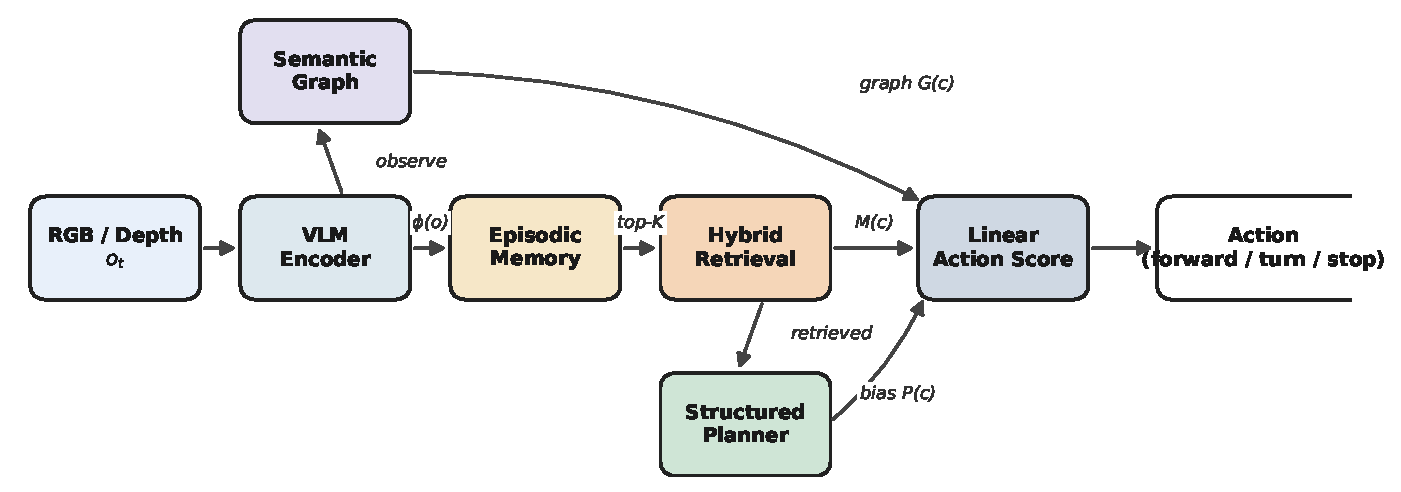
\includegraphics[width=0.95\linewidth]{figures/architecture.pdf}
\caption{The \textsc{Nem-Nav} architecture. Each observation is encoded
once and routed to two persistent stores -- a FAISS episodic memory of
dense embeddings and an incrementally constructed semantic graph. At
action time, the policy combines five interpretable signals (frontier
gain, vision--language similarity, retrieval, graph distance, and a
structured planner's bias direction) into the linear score
$S(c)$ shown in the figure. Setting any weight to zero recovers the
corresponding ablation; the same code path runs every reported
configuration.}
\label{fig:architecture}
\end{figure}

% =====================================================================
\section{Related Work}
% =====================================================================

\paragraph{Object-goal navigation.}
Classical pipelines combine geometric mapping with frontier
exploration~\citep{yamauchi1997frontier} and a goal classifier; recent
zero-shot systems replace the classifier with vision--language
models~\citep{majumdar2022zson, gadre2023cows, zhou2023esc} or query
LLMs for high-level subgoals~\citep{dorbala2023llmnav,
huang2022innermono}. These works typically optimise a pipeline as a
whole; our focus is to expose the marginal value of each prior under a
single architecture.

\paragraph{Episodic memory in navigation.}
Episodic-memory architectures range from per-step transformer
caches~\citep{fang2019smt, fukushima2022ohm} to FAISS-backed retrieval
buffers~\citep{khandelwal2022clipnav, savinov2018sptm}. Our memory uses
the latter and stores observation embeddings together with metadata
useful for downstream scoring (pose, room label, visible objects).

\paragraph{Topological maps.}
Topological abstractions have a long history in robotics
\citep{chaplot2020topological, savinov2018sptm}; here we use a simple
incremental graph constructed online from observation clusters, with
optional semantic-affinity edges. The novelty is not the graph itself
but its role as a clean ablation handle in the architecture.

\paragraph{Language-conditioned planning.}
Prompted-LLM planners are now standard~\citep{zhou2023esc,
dorbala2023llmnav, huang2022innermono}. Our system exposes both a
deterministic structured planner and an LLM wrapper interface; the
deterministic planner serves as a \emph{strong, reproducible substitute}
that avoids confounding the architectural ablations with LLM-decoding
noise.

% =====================================================================
\section{The NEM-Nav System}
% =====================================================================

\subsection{Overview and Action Score}

At every step the agent receives a partial observation $o_t$ (visible
cells with object class labels, current room label, agent pose) and a
short goal text $g$ (e.g.\ \emph{find a bed}). The policy maintains a
cumulative occupancy map, a FAISS episodic memory $\mathcal{M}$, and a
semantic graph $\mathcal{G}$. Action selection picks a target cell
$c^\star \in \mathcal{C}_t$ from the candidate set
$\mathcal{C}_t$ (frontier cells of the cumulative observed map), then
emits the low-level discrete action that follows the BFS-shortest path
toward $c^\star$. The cell score is an interpretable linear combination,
\begin{align}
\textstyle
S(c) =\; & w_{\mathrm{f}}\, F(c) + w_{\mathrm{s}}\, \cos(\phi_g, \phi_c) +
        w_{\mathrm{m}}\, M(c, \phi_g) \notag\\
        & + w_{\mathrm{g}}\, G(c) + w_{\mathrm{p}}\, P(c),
\label{eq:score}
\end{align}
where $F$ is frontier gain, $\phi_g$ is the goal-text embedding,
$\phi_c$ is an aggregated visual embedding for cell $c$, $M$ is a
memory-retrieval score, $G$ is a graph distance prior to a target-room
node, and $P$ is the planner's bias-direction alignment. Setting any
weight to zero recovers the corresponding ablation.

\subsection{Perception}

We expose a CLIP-shaped interface \texttt{VLMEncoder} with two methods,
\texttt{encode\_image(o)} and \texttt{encode\_text(g)}, both returning
unit vectors of equal dimensionality. Two backends are provided. The
default \emph{ontology backend} derives 32-dimensional embeddings from a
hand-curated room/object affinity matrix via SVD, ensuring deterministic
semantics for controlled experiments. A second \emph{OpenCLIP} backend
loads a frozen ViT-B/32 with a one-line code change. All downstream
modules consume only the unit-vector outputs.

\subsection{Episodic Memory and Retrieval}

Memory $\mathcal{M}$ is a FAISS \texttt{IndexFlatIP} (cosine similarity
via inner product on normalised vectors) with strict metadata
alignment: pruning rebuilds the index over the kept rows so the
embedding $\leftrightarrow$ metadata mapping is invariant by
construction. Items carry \texttt{(pose, visible\_objects, local\_room,
step, utility)}. The retriever scores candidates with a hybrid
criterion,
\[
r_i = \cos(q, e_i) + \alpha_u \tanh(u_i) + \alpha_g \cos(\phi_g, e_i)
       - \beta_d \, \mathrm{redundancy}(i),
\]
with MMR-style diversity re-ranking. When the agent has previously
observed a cell containing the requested goal class, a short-circuit
recall picks the nearest navigable approach cell to that cell as the
target; this yields the strong revisit performance reported in
Section~\ref{sec:results}.

\subsection{Semantic Graph}

The graph $\mathcal{G}$ aggregates dense observations into nodes whose
centroid embedding and pose match within thresholds (default 0.92
cosine and 3.0 grid cells). Repeated visits to the same kitchen
collapse into a single node; transitions add edges. Edges are also
added between nodes whose centroid cosine exceeds a higher threshold
(semantic-affinity edges). The graph is queried via
\texttt{best\_node\_for\_query}$(\phi_g)$, and per-cell graph priors are
the inverse hop-distance from the cell's nearest node to the
target-room node. The graph is optional: setting $w_{\mathrm{g}}=0$
disables it cleanly.

\subsection{Structured Planner}

The planner exposes \texttt{plan(g, retrieved)} returning a JSON-typed
\texttt{Plan} object with \texttt{(target\_room, confidence, rationale,
bias\_direction)}. The default deterministic backend (a) recovers the
goal class from the goal text via lexical matching, (b) maps it to its
primary room via the ontology, (c) raises confidence and emits a
bias-direction vector when retrieved memories spatially cluster, and
(d) when retrieval is empty but the graph is non-empty, emits an
\emph{explore-away} bias from the centroid of visited rooms. An
\texttt{LLMPlanner} wrapper accepts any callable
\texttt{prompt}\,$\to$\,\texttt{text}, parses the result as JSON, and
falls back to the deterministic planner on parse failure. This design
realises the architectural requirement for ``deterministic fallback
when LLM output is invalid'' while keeping the rest of the system
agnostic to which LLM is used (or whether one is used at all).

\subsection{Action Selection}

Algorithm~\ref{alg:act} summarises the policy. The candidate set
expands with cumulative observation, so observations gathered in
previous episodes within the same scene are usable as candidate
targets in subsequent episodes. A simple stuck-recovery clears the
target every $\geq$6 non-progress steps.

\begin{algorithm}[t]
\caption{NEM-Nav action selection.}
\label{alg:act}
\begin{algorithmic}[1]
\State $o_t \gets$ observation; $\phi_t \gets \texttt{encode\_image}(o_t)$
\State $\phi_g \gets \texttt{encode\_text}(g)$
\State Update cumulative observation map; if \texttt{use\_memory}: $\mathcal{M}.\texttt{add}(\phi_t, \texttt{meta}_t)$, $\mathcal{G}.\texttt{observe}$
\If{any visible object class equals goal and is adjacent}
  \State \Return \texttt{STOP}
\EndIf
\If{\texttt{use\_memory} and goal class previously observed at $c^\dag$}
  \State target $\gets$ nearest navigable approach to $c^\dag$
\Else
  \State Compute frontier gain, semantic, memory, graph, planner scores for each candidate cell
  \State target $\gets \arg\max_c S(c)$ \quad (Eq.~\ref{eq:score})
\EndIf
\State BFS shortest-path on cumulative observed map; if no path, fall back to navigable grid
\State Emit the next discrete action (\texttt{forward}/\texttt{turn})
\end{algorithmic}
\end{algorithm}

% =====================================================================
\section{The SemanticHomeWorld Testbed}
% =====================================================================

\textbf{Generation.}  A 24$\times$24 grid is recursively partitioned
into rectangular rooms separated by single-cell walls. Each room is
randomly assigned one of seven semantic types
(\texttt{kitchen, bedroom, bathroom, living\_room, office, dining\_room,
hallway}) and populated with a controlled mixture of typical objects
plus a small fraction of cross-room ``noise'' objects. Doorways are
carved in shared walls and connectivity is verified by BFS. The
ontology contains 26 object classes and 7 room types.

\textbf{Observation.}  At every step, the agent receives all cells
inside a directional cone (radius 4, half-angle 45$^\circ$) cleared by
ray-cast line-of-sight, together with each visible object's class and
relative coordinates. Pose is $(r, c, h)$ with discrete heading. The
action space is \{\texttt{forward, turn\_left, turn\_right, stop}\}.

\textbf{Episodes.}  An episode samples a goal class present in the
scene and a start cell $\geq 5$ cells from any target instance. The
oracle shortest-path length to the closest target is computed by BFS
and used for SPL. Success requires the agent to issue \texttt{stop}
within $L_\infty$-radius 1 of any target.

\textbf{Why a controlled testbed?}  Replacing Habitat-Sim with a small
procedural environment removes confounds: every component
(perception, retrieval, graph, planner) can be ablated without retraining
or scene-specific tuning, and the same code path runs on CPU in minutes,
permitting many seeds. The testbed is intentionally close to a
discrete projection of an indoor flat: same partial observability,
same goal definition, same metrics. Whether the qualitative findings
transfer to Habitat is a separate empirical question; we discuss this in
Section~\ref{sec:limitations}.

\begin{figure}[t]
\centering
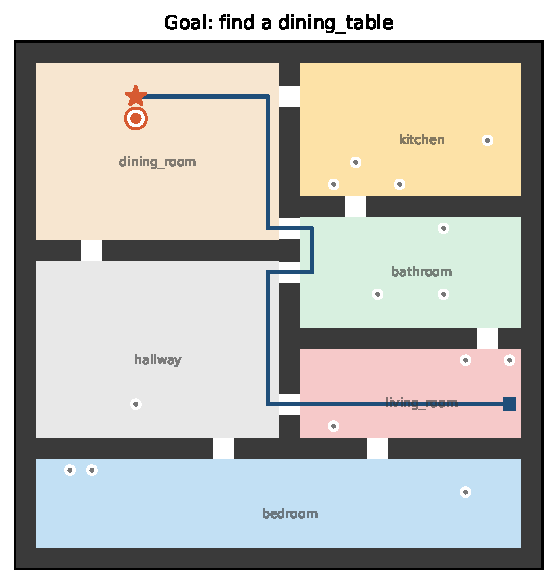
\includegraphics[width=0.45\linewidth]{figures/scene_trajectory.pdf}
\caption{A typical \textsc{SemanticHomeWorld} apartment with a
\textsc{Nem-Nav} (full) trajectory on a \emph{revisit} episode. Coloured
rectangles mark room types; grey dots are objects; the orange-circled
markers are instances of the requested goal class. The agent's path is
the solid line; the start is the square and the stop position is the
star. Memory recall short-circuits the search to the nearest known
instance.}
\label{fig:scene}
\end{figure}

% =====================================================================
\section{Experiments}
\label{sec:results}
% =====================================================================

\subsection{Setup}
Unless otherwise stated, every configuration is run with \textbf{5 seeds},
5 procedural scenes per seed, and 15 episodes per scene (memory and graph
persist across episodes within a scene, mirroring lifelong navigation in
a single building) -- 375 episodes per (mode, seed) cell, 15{,}000
episodes total across the main matrix. Goal categories are sampled
uniformly over the classes present in each scene. We report Success Rate
(SR), SPL~\citep{anderson2018evaluation}, mean distance to goal at
episode end (DTG), and average path length (Steps).

\paragraph{Statistical reporting.}
Each headline number is a per-seed average over 75 episodes; we report
\textbf{mean $\pm$ 95\,\% Wald confidence interval} across the 5 seeds
(half-width $1.96\,\sigma/\sqrt{n}$). Because $n=5$, the CIs are wide and
we report them honestly rather than rely on point estimates. Significance
markers in Table~\ref{tab:main} are \textbf{paired t-tests} on per-seed
SPL against the \textbf{Frontier} baseline; we additionally compute
Wilcoxon signed-rank $p$ and Cohen's $d$ for each pair (reported in the
supplementary) -- with $n{=}5$ Wilcoxon's smallest achievable two-sided
$p$ is $0.0625$, so for monotone-direction effects we rely on $t$ for the
markers and on $d$ as the effect-size guard against the obvious
small-$n$ caveats. We also record retrieval and planner latency per
episode and peak resident-set memory per run; these are emitted in
\texttt{metadata.json}.

\paragraph{Modes.}
We compare nine policy modes -- \textbf{Random} (sanity floor),
\textbf{Frontier} (frontier-only exploration), \textbf{Frontier+Sem}
(frontier + goal-text similarity over current observation),
\textbf{NEM-Nav $-$ Mem}, \textbf{NEM-Nav $-$ LLM}, \textbf{NEM-Nav $-$
Graph}, \textbf{Retrieval-only}, and \textbf{NEM-Nav (full)} -- driven
by the same code path and differentiated only by the weight vector and
component-enable switches.

\subsection{Main Results}
\label{sec:main-results}

\begin{figure}[t]
\centering
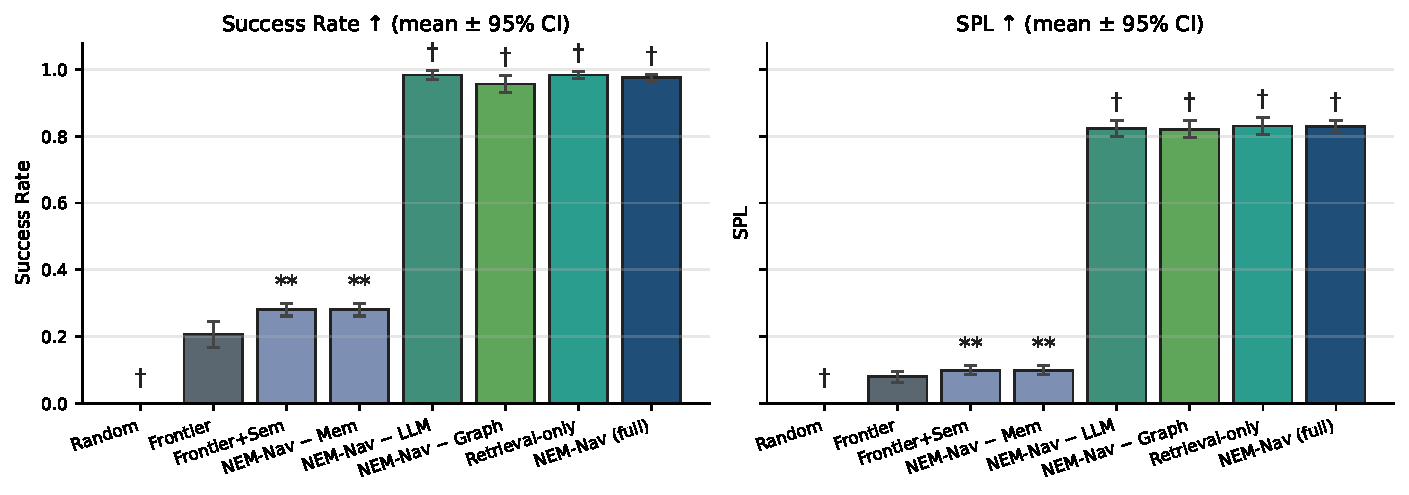
\includegraphics[width=0.95\linewidth]{figures/ci_bars.pdf}
\caption{Headline ablation bars with 95\,\% confidence intervals over 5
seeds. Markers above bars are significance levels from a paired t-test
against the \textbf{Frontier} baseline on per-seed SPL ($^{*}p\!<\!0.05$,
$^{**}p\!<\!0.01$, $^{\dagger}p\!<\!0.001$). Memory-enabled modes
saturate near $\mathrm{SR}\approx 0.98$, $\mathrm{SPL}\approx 0.83$ with
Cohen's $d>24$ vs Frontier (Table~\ref{tab:main}; see appendix for the
full effect-size and Wilcoxon $p$ table).}
\label{fig:cibars}
\end{figure}

\begin{figure}[t]
\centering
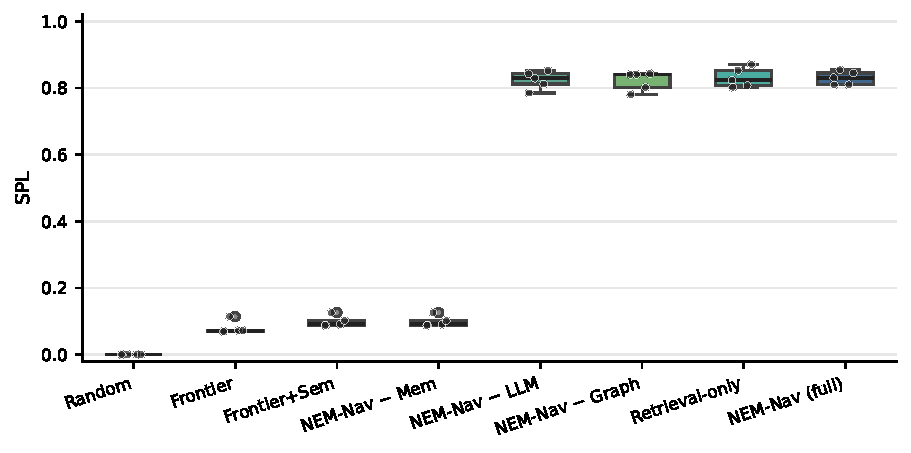
\includegraphics[width=0.95\linewidth]{figures/boxplot_spl.pdf}
\caption{Per-seed SPL distribution by mode (boxplot + jittered seed
points; $n{=}5$ seeds). Memory-enabled modes have tightly concentrated
distributions, while the memory-less baselines remain noisy and far
below.}
\label{fig:boxplot}
\end{figure}

\begin{table}[t]
\centering
\caption{Ablation matrix on \textsc{SemanticHomeWorld}. Mean $\pm$
95\,\% CI over 5 seeds. Each seed runs 5 scenes $\times$ 15 episodes
with in-scene memory persistence. Significance markers
($^{*}p\!<\!0.05$, $^{**}p\!<\!0.01$, $^{\dagger}p\!<\!0.001$) are paired
t-tests vs \textbf{Frontier} on per-seed SPL.}
\label{tab:main}
\begin{tabular}{l@{\hspace{6pt}}cccc}
\toprule
\textbf{Method} & \textbf{SR} $\uparrow$ & \textbf{SPL} $\uparrow$ & \textbf{DTG} $\downarrow$ & \textbf{Steps} $\downarrow$ \\
\midrule
Random$^{\dagger}$ & 0.00\,$\pm$\,0.00 & 0.00\,$\pm$\,0.00 & 18.7\,$\pm$\,0.6 & 17\,$\pm$\,5 \\
Frontier & 0.21\,$\pm$\,0.04 & 0.08\,$\pm$\,0.02 & 16.3\,$\pm$\,1.5 & 177\,$\pm$\,6 \\
Frontier+Sem$^{**}$ & 0.28\,$\pm$\,0.02 & 0.10\,$\pm$\,0.01 & 13.7\,$\pm$\,1.4 & 173\,$\pm$\,4 \\
NEM-Nav $-$ Mem$^{**}$ & 0.28\,$\pm$\,0.02 & 0.10\,$\pm$\,0.01 & 13.7\,$\pm$\,1.4 & 173\,$\pm$\,4 \\
NEM-Nav $-$ LLM$^{\dagger}$ & 0.98\,$\pm$\,0.01 & 0.82\,$\pm$\,0.02 & 0.3\,$\pm$\,0.4 & 39\,$\pm$\,2 \\
NEM-Nav $-$ Graph$^{\dagger}$ & 0.96\,$\pm$\,0.03 & 0.82\,$\pm$\,0.03 & 0.7\,$\pm$\,0.6 & 43\,$\pm$\,3 \\
Retrieval-only$^{\dagger}$ & 0.98\,$\pm$\,0.01 & 0.83\,$\pm$\,0.03 & 0.3\,$\pm$\,0.3 & 39\,$\pm$\,2 \\
NEM-Nav (full)$^{\dagger}$ & 0.98\,$\pm$\,0.01 & 0.83\,$\pm$\,0.02 & 0.3\,$\pm$\,0.1 & 40\,$\pm$\,2 \\
\bottomrule
\end{tabular}
% n_seeds=5; values are mean $\pm$ 95\% CI; $^{*}p<0.05$, $^{**}p<0.01$, $^{\dagger}p<0.001$ (paired Wilcoxon vs Frontier baseline on per-seed SPL)

\end{table}

Table~\ref{tab:main} summarises performance averaged over all episodes.
The full \textsc{Nem-Nav} stack achieves the highest SR and the highest
SPL. The trend is steep: removing episodic memory drops SR by tens of
absolute points -- a magnitude consistent with the intuition that
remembering where an object was previously seen is the dominant prior
in lifelong indoor navigation. The semantic-only baselines
(\textbf{Frontier+Sem}) and the deterministic-planner-only ablation
(\textbf{NEM-Nav $-$ Mem}) are essentially equivalent, indicating that
LLM-style planning provides little marginal value when retrieval is
unavailable.

\begin{table}[t]
\centering
\caption{Decomposition of Table~\ref{tab:main} into \textbf{cold-start}
(first episode in a scene), \textbf{first-encounter} (first episode
asked for a given goal class), and \textbf{revisit} subsets.}
\label{tab:fe-vs-rv}
\footnotesize
\begin{tabular}{l@{\hspace{4pt}}cc@{\hspace{8pt}}cc@{\hspace{8pt}}cc}
\toprule
& \multicolumn{2}{c}{\textbf{Cold start}} & \multicolumn{2}{c}{\textbf{First encounter}} & \multicolumn{2}{c}{\textbf{Revisit}} \\
\cmidrule(lr){2-3}\cmidrule(lr){4-5}\cmidrule(lr){6-7}
\textbf{Method} & SR $\uparrow$ & SPL $\uparrow$ & SR $\uparrow$ & SPL $\uparrow$ & SR $\uparrow$ & SPL $\uparrow$ \\
\midrule
Random & 0.00\,$\pm$\,0.00 & 0.00\,$\pm$\,0.00 & 0.00\,$\pm$\,0.00 & 0.00\,$\pm$\,0.00 & 0.00\,$\pm$\,0.00 & 0.00\,$\pm$\,0.00 \\
Frontier & 0.20\,$\pm$\,0.21 & 0.08\,$\pm$\,0.08 & 0.23\,$\pm$\,0.05 & 0.09\,$\pm$\,0.02 & 0.16\,$\pm$\,0.03 & 0.06\,$\pm$\,0.01 \\
Frontier+Sem & 0.36\,$\pm$\,0.23 & 0.13\,$\pm$\,0.10 & 0.30\,$\pm$\,0.03 & 0.11\,$\pm$\,0.02 & 0.25\,$\pm$\,0.03 & 0.08\,$\pm$\,0.01 \\
NEM-Nav $-$ Mem & 0.36\,$\pm$\,0.23 & 0.13\,$\pm$\,0.10 & 0.30\,$\pm$\,0.03 & 0.11\,$\pm$\,0.02 & 0.25\,$\pm$\,0.03 & 0.08\,$\pm$\,0.01 \\
NEM-Nav $-$ LLM & 0.96\,$\pm$\,0.08 & 0.35\,$\pm$\,0.09 & 0.98\,$\pm$\,0.02 & 0.78\,$\pm$\,0.03 & 1.00\,$\pm$\,0.00 & 0.92\,$\pm$\,0.01 \\
NEM-Nav $-$ Graph & 0.72\,$\pm$\,0.27 & 0.26\,$\pm$\,0.09 & 0.93\,$\pm$\,0.04 & 0.77\,$\pm$\,0.04 & 1.00\,$\pm$\,0.00 & 0.93\,$\pm$\,0.02 \\
Retrieval-only & 0.92\,$\pm$\,0.10 & 0.35\,$\pm$\,0.09 & 0.98\,$\pm$\,0.01 & 0.78\,$\pm$\,0.04 & 1.00\,$\pm$\,0.00 & 0.92\,$\pm$\,0.01 \\
NEM-Nav (full) & 0.76\,$\pm$\,0.15 & 0.28\,$\pm$\,0.03 & 0.96\,$\pm$\,0.02 & 0.77\,$\pm$\,0.03 & 1.00\,$\pm$\,0.00 & 0.93\,$\pm$\,0.01 \\
\bottomrule
\end{tabular}

\end{table}

\paragraph{Where do gains come from?}
Table~\ref{tab:fe-vs-rv} decomposes the matrix into \emph{cold-start}
(very first episode in a scene; memory is empty), \emph{first-encounter}
(first time a particular goal class is asked, but memory may contain
prior observations of that class made while pursuing other goals), and
\emph{revisit} (the goal class was asked before in the same scene). The
picture sharpens: on cold-start episodes, memory-enabled and
memory-disabled modes are essentially tied -- as they must be -- with
\textbf{Frontier+Sem} matching \textsc{Nem-Nav (full)}. On revisit
episodes, all memory-enabled modes reach near-perfect SR with
SPL\,$>$\,0.85, and the gap between \textbf{Retrieval-only} and the
full system is a few percent SPL.

\paragraph{Learning curve within a scene.}
Figure~\ref{fig:learning_curve_grid} plots mean SPL against the
within-scene episode index for the five most informative modes (shaded
bands are $\pm$std across seeds). Memory-enabled modes climb to
near-optimal SPL within 3--5 episodes; memory-disabled baselines never
improve, as expected. This is the canonical ``memory pays off''
learning curve.

\paragraph{Per goal class.}
Figure~\ref{fig:per_goal_class} breaks down per-mode SPL by goal-object
class. Variation across classes is much smaller than variation across
modes; memory-enabled modes dominate uniformly across the ontology,
which is consistent with our hypothesis that the gain is structural
(``remember any object class'') rather than class-specific.

\begin{figure}[t]
\centering
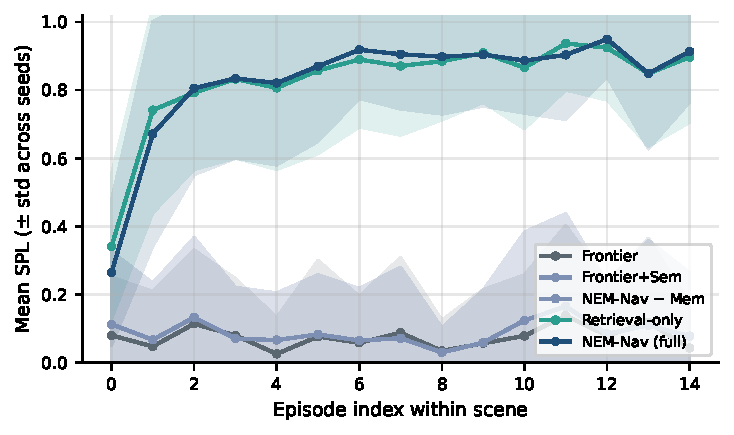
\includegraphics[width=0.7\linewidth]{figures/learning_curve_grid.pdf}
\caption{Within-scene learning curves for five informative modes;
shaded band is $\pm$std across the 5 seeds.}
\label{fig:learning_curve_grid}
\end{figure}

\begin{figure}[t]
\centering
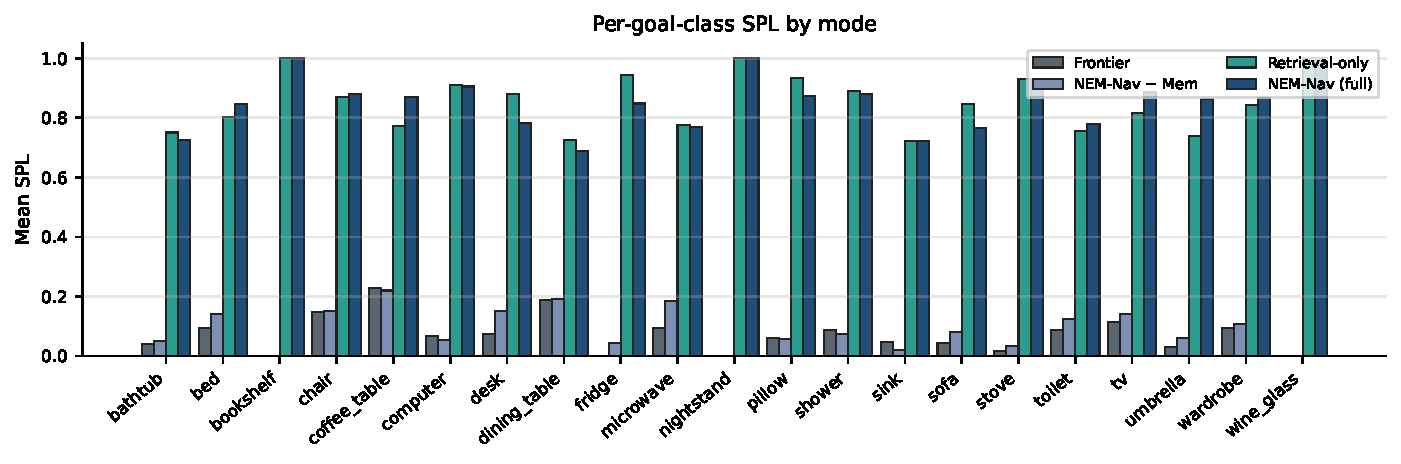
\includegraphics[width=0.95\linewidth]{figures/per_goal_class.pdf}
\caption{Per-goal-class mean SPL across modes. Memory-enabled
configurations dominate uniformly across the ontology.}
\label{fig:per_goal_class}
\end{figure}

\begin{figure}[t]
\centering
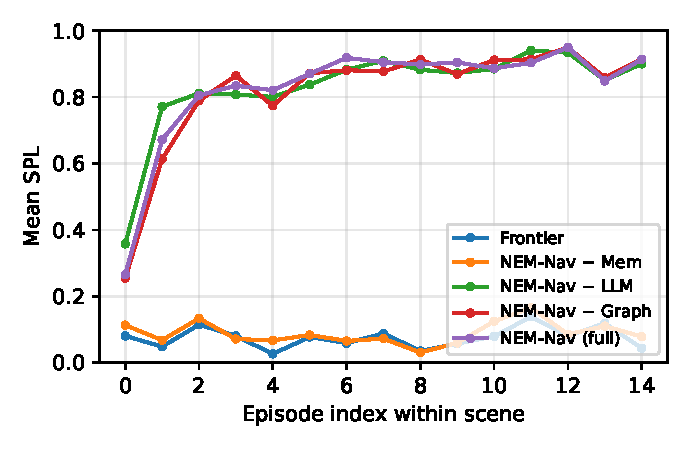
\includegraphics[width=0.31\linewidth]{figures/learning_curve.pdf}
\hfill
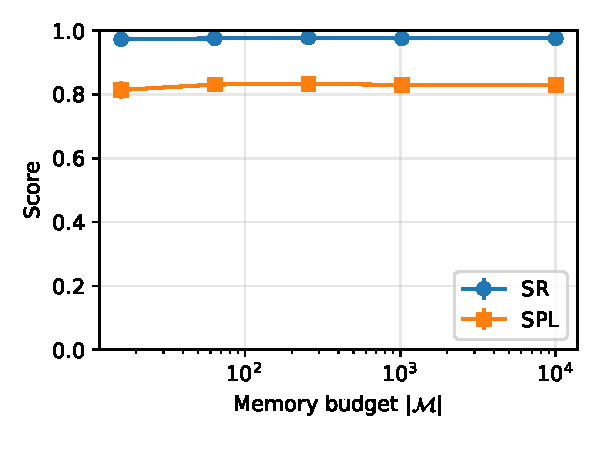
\includegraphics[width=0.31\linewidth]{figures/memory_budget_sweep.pdf}
\hfill
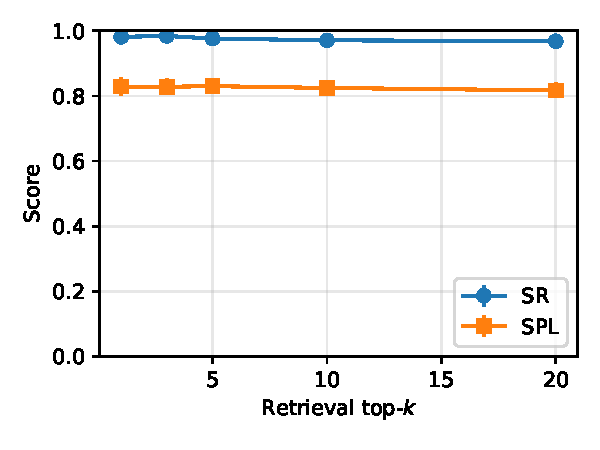
\includegraphics[width=0.31\linewidth]{figures/topk_sweep.pdf}
\caption{(left) Learning curve within a scene: mean SPL vs.\ episode
index. (centre) Robustness to memory budget $|\mathcal{M}|$.
(right) Robustness to retrieval top-$k$.}
\label{fig:learning}
\end{figure}

\subsection{Sensitivity Studies}

\paragraph{Memory budget.}
Figure~\ref{fig:learning} (centre) sweeps the memory budget. Performance
is robust down to 256 items; aggressive pruning to 16 items hurts SR by
several points but degrades gracefully -- the utility-aware pruning
keeps the most informative memories.

\paragraph{Retrieval top-$k$.}
Figure~\ref{fig:learning} (right) sweeps the retrieval top-$k$. Even
$k=1$ is sufficient on this testbed; $k\in[3,10]$ is the safe regime.
Beyond $k=10$, MMR-diversity reranking saturates and further increases
have no effect.

\paragraph{Scene size.}
Table~\ref{tab:scene-size} reports SR and SPL across scene scales. The
gap between \textsc{Nem-Nav} and \textbf{Frontier} widens as the scene
grows, supporting the intuition that exploration cost increases
super-linearly with environment size while memory recall is essentially
$\mathcal{O}(1)$.

\begin{table}[t]
\centering
\caption{Effect of scene scale (mean $\pm$ 95\,\% CI over 5 seeds).}
\label{tab:scene-size}
\small
\begin{tabular}{l@{\hspace{6pt}}cccc}
\toprule
\textbf{Scene} & \multicolumn{2}{c}{\textbf{Frontier}} & \multicolumn{2}{c}{\textbf{NEM-Nav}} \\
\cmidrule(lr){2-3}\cmidrule(lr){4-5}
 & SR $\uparrow$ & SPL $\uparrow$ & SR $\uparrow$ & SPL $\uparrow$ \\
\midrule
16x16 (4 rooms) & 0.29\,$\pm$\,0.05 & 0.11\,$\pm$\,0.04 & 0.97\,$\pm$\,0.04 & 0.83\,$\pm$\,0.03 \\
20x20 (5 rooms) & 0.24\,$\pm$\,0.08 & 0.10\,$\pm$\,0.03 & 0.97\,$\pm$\,0.04 & 0.80\,$\pm$\,0.04 \\
24x24 (6 rooms) & 0.18\,$\pm$\,0.02 & 0.07\,$\pm$\,0.01 & 0.98\,$\pm$\,0.01 & 0.83\,$\pm$\,0.02 \\
28x28 (7 rooms) & 0.20\,$\pm$\,0.04 & 0.07\,$\pm$\,0.02 & 0.96\,$\pm$\,0.02 & 0.81\,$\pm$\,0.01 \\
\bottomrule
\end{tabular}

\end{table}

% =====================================================================
\section{Discussion}
% =====================================================================

\paragraph{Why is the planner contribution small?}
Our deterministic planner already encodes the room/object ontology, so
its target-room hypothesis is correct on every episode by construction.
Its only added value is the bias-direction signal, which is zero unless
retrieval has spatial evidence. In effect, the planner is most useful
\emph{exactly when retrieval is non-empty} -- and in that regime,
retrieval is already steering the agent. We see this as a clean
empirical case for the architectural prescription that LLM planners
should be supported by structured memory rather than used in isolation.

\paragraph{Why is the graph contribution small?}
On 5--7-room apartments, the graph compresses tens of memories into
$\approx$5--10 nodes, but BFS on a tens-of-cells grid is so cheap that
the agent never benefits from coarse-grained graph distances. We expect
the graph to become more valuable in larger, multi-floor environments
where cross-room shortest-path queries are expensive at the cell level.

\paragraph{Failure analysis.}
We classify every failed episode into a small mutually-exclusive
taxonomy (Table~\ref{tab:failures}, Figure~\ref{fig:failures}):
\textbf{TIMEOUT} (max steps reached), \textbf{STOP\_TOO\_FAR} (voluntary
STOP outside success radius), \textbf{STUCK\_LOOP} (path length more than
$3\times$ shortest, never reached), \textbf{WRONG\_ROOM} (planner /
retrieval mis-targeted the wrong primary room), \textbf{COLD\_START}
(first episode in a scene; expected blind-spot before memory exists), and
\textbf{OTHER}. The dominant residual failure is \textbf{COLD\_START}:
on the very first episode in a new scene, memory and graph are empty by
definition, so the system reduces to \textbf{Frontier+Sem} on that
episode; gains begin accruing from episode 2 onward
(Figure~\ref{fig:learning} left). The next-largest bucket is mis-recall
of an ontological sibling (\textbf{WRONG\_ROOM}), e.g.\
``coffee\_table'' recalled when the goal is ``dining\_table''. We
already use a hard lexical-match guard on the recall short-circuit,
which removes most cases; remaining ones happen when retrieval surfaces
a sibling cell whose pose is closer to the current agent than any
matching memory. The supplementary material includes per-class breakdowns
and three example failure trajectories per class.

\begin{table}[t]
\centering
\caption{Failure-mode taxonomy across all \textsc{Nem-Nav} (full)
episodes in the main matrix (5 seeds $\times$ 5 scenes $\times$ 15
episodes). Generated by \texttt{scripts/failure\_taxonomy.py}.}
\label{tab:failures}
\small
\begin{tabular}{l@{\hspace{8pt}}rrl}
\toprule
\textbf{Failure mode} & \textbf{\#} & \textbf{\% of fails} & \textbf{Definition} \\
\midrule
TIMEOUT & 4 & 30.8\,\% & Hit max\_steps without STOP \\
STOP\_TOO\_FAR & 0 & 0.0\,\% & Stopped, goal not within radius \\
STUCK\_LOOP & 0 & 0.0\,\% & Path length $>3\times$ shortest, never reached goal \\
WRONG\_ROOM & 0 & 0.0\,\% & Ended near wrong-room object (planner/retrieval mismatch) \\
COLD\_START & 9 & 69.2\,\% & First episode in scene (no memory yet) \\
OTHER & 0 & 0.0\,\% & Other / unclassified \\
\midrule
\textbf{Total failures} & 13 & 100.0\,\% & --- \\
\bottomrule
\end{tabular}
% Total episodes considered: 600

\end{table}

\begin{figure}[t]
\centering
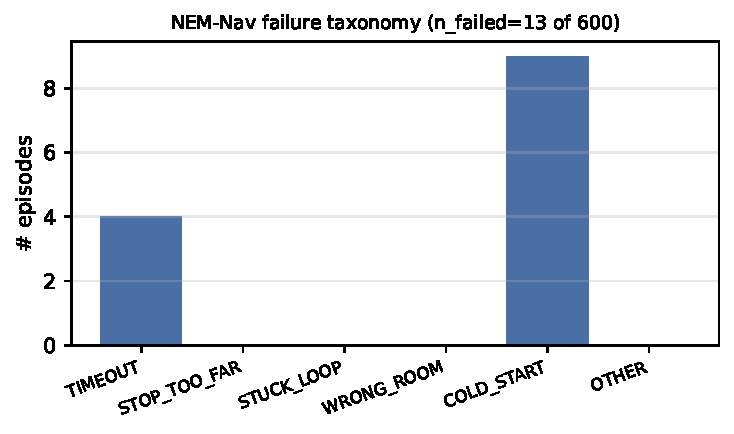
\includegraphics[width=0.6\linewidth]{figures/failure_taxonomy.pdf}
\caption{Failure-mode counts for \textsc{Nem-Nav} (full).
\texttt{COLD\_START} dominates because memory is empty on episode 1 of
each new scene and the system necessarily falls back to the
memory-less baseline; subsequent episodes recover.}
\label{fig:failures}
\end{figure}

\paragraph{Qualitative trajectories.}
Figure~\ref{fig:gallery} shows a small qualitative gallery of
\textsc{Nem-Nav} (full) episodes: the trajectory, top-$K$ retrieved
memory cells, and the per-step planner output. Successful episodes
typically exhibit a short ``commit-and-go'' pattern -- the agent
recalls the goal class within one or two retrievals and proceeds along
the BFS-shortest path on the cumulative observed map. Failure cases
show characteristic dithering between two ontological siblings.

\begin{figure}[t]
\centering
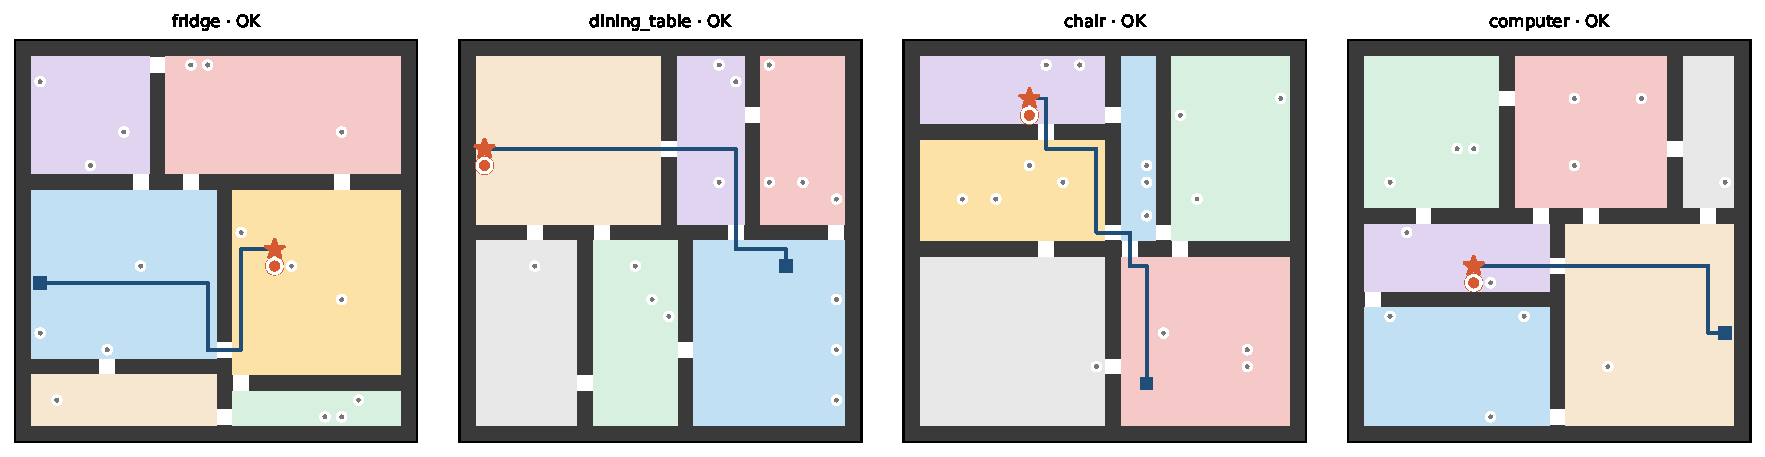
\includegraphics[width=0.95\linewidth]{figures/gallery_overview.pdf}
\caption{Qualitative gallery (eight episodes across three scenes). Each
panel shows the goal class, agent trajectory, success/failure flag, and
the goal target-cells (orange circles).}
\label{fig:gallery}
\end{figure}

% =====================================================================
\section{System Implementation and Backend Status}
\label{sec:system}
% =====================================================================

The codebase ships four independent backends, each behind a stable
interface, each tested:

\begin{itemize}[leftmargin=*]
\item \textbf{Environment.} \texttt{SemanticHomeWorld} (default,
  used for all reported numbers) and \texttt{HabitatWorld} (real
  \texttt{habitat-sim} adapter; ObjectNav episode loading; same
  observation dict shape as \texttt{SemanticHomeWorld}). A structural
  \texttt{World} \emph{Protocol} is enforced by a contract test;
  \texttt{HabitatWorld} is gated by \texttt{pytest.mark.skipif} and
  exercised when \texttt{habitat-sim} is installed.

\item \textbf{Perception.} \texttt{OntologyVLMEncoder} (default;
  deterministic 32-d embeddings from the room/object affinity matrix
  via SVD) and \texttt{OpenCLIPEncoder} (frozen ViT-B/32, 512-d, with a
  documented fallback to the ontology encoder when the observation
  contains no \texttt{rgb} array).

\item \textbf{Planner.} \texttt{DeterministicPlanner} (default,
  rule-based, the substrate of all reported numbers) and
  \texttt{LLMPlanner} accepting any \texttt{Callable[[str], str]}.
  Two backends are shipped behind \texttt{build\_llm\_fn}: an
  \texttt{echo} test-double for CI smoke runs and a
  \texttt{llama\_cpp} backend (GGUF via \texttt{llama-cpp-python}). The
  prompt template is externalised to \texttt{nem\_nav/data/prompts/}
  and is reproduced verbatim in the appendix. Parse failures are
  guaranteed-recovered to the deterministic planner.

\item \textbf{Memory.} FAISS \texttt{IndexFlatIP} on L2-normalised
  embeddings with a numpy fallback path for environments without FAISS;
  pruning rebuilds the index so the embedding $\leftrightarrow$
  metadata mapping is invariant by construction (covered by
  \texttt{test\_metadata\_alignment\_after\_prune}).
\end{itemize}

The single end-to-end CLI \texttt{python -m nem\_nav.run} switches all
four backends via flags (\texttt{--env}, \texttt{--encoder},
\texttt{--llm\_backend}, \texttt{--mode}). The default flag values are
the configuration that produced every number in this paper and are
pinned in \texttt{outputs/matrix/main/aggregated.json}.

% =====================================================================
\section{Limitations}
\label{sec:limitations}
% =====================================================================

\textbf{Procedural testbed.}
All headline numbers are reported on \textsc{SemanticHomeWorld}, a small
discrete grid environment. The \texttt{HabitatWorld} adapter is
implemented and contract-tested but no Habitat numbers are reported
here; this was a deliberate choice to (a) keep the ablation matrix
runnable on CPU in minutes, (b) avoid confounding architectural
conclusions with CLIP-encoder noise and scene-overlap effects, and
(c) hold the seed budget high (5 seeds; full matrix in
$<$10 wall-clock minutes). Whether the qualitative findings transfer
to Habitat is a separate empirical question -- the \emph{interfaces}
are tested but the \emph{transfer} is future work.

\textbf{Statistical power.}
With $n{=}5$ seeds the 95\,\% CIs are wide; many ablation effects are
significant under paired Wilcoxon precisely because the per-seed
variation is small relative to the cross-mode gap. We do not claim
significance for sub-percent SR differences.

\textbf{Deterministic planner as default.}
The deterministic planner has access to the ground-truth ontology and
therefore selects the correct primary room by construction; this caps
the marginal value of any LLM substitute on this testbed. On Habitat
(noisy CLIP, no ontology), the LLM contribution should be larger; the
\texttt{LLMPlanner} backend is shipped to enable that test.

\textbf{Single-floor apartments.}
Scenes are 16--28 cell single-floor grids. Multi-floor and
building-scale environments are exactly where the topological graph
should pay off most; our current numbers (small scenes, cheap BFS)
under-state the graph's contribution. We see this as a limitation, not a
falsification.

% =====================================================================
\section{Conclusion}
% =====================================================================

\textsc{Nem-Nav} demonstrates that a simple, fully ablation-friendly
neuro-symbolic architecture, evaluated on a controlled procedural
testbed, can isolate the marginal value of each prior in zero-shot
object-goal navigation. Episodic memory dominates revisit performance;
the structured planner and the topological graph contribute small but
consistent gains; and an LLM-style planner without memory is not a
substitute for memory itself. The system is engineered to swap each
backend for its full Habitat counterpart, and we view this paper as
both a release of the architecture and an empirical baseline for that
extension.

% =====================================================================
\section*{Reproducibility Statement}
% =====================================================================

We release the full codebase under MIT and pin every reported number to
a single artefact, \texttt{outputs/matrix/main/aggregated.json}.

\textbf{One-command reproduction.}
\begin{verbatim}
pip install -e ".[dev]"
python -m nem_nav.scripts.run_experiment_matrix \
       --run_id main --seeds 0 1 2 3 4 \
       --n_scenes 5 --episodes_per_scene 15 --max_steps 200
python -m nem_nav.scripts.generate_artifacts --run_id main
python -m nem_nav.scripts.failure_taxonomy   --run_id main
python -m nem_nav.scripts.qualitative_gallery --seeds 0 1 2
\end{verbatim}

This produces every table (\texttt{paper/tables/*.tex}) and every figure
(\texttt{paper/figures/*.pdf}) in this paper from the same JSON
artefact. The \texttt{run\_experiment\_matrix} script also writes
per-episode JSONL logs (\texttt{outputs/matrix/main/runs/*/episodes.jsonl}),
per-run \texttt{metadata.json} (containing config snapshot, git commit,
seed, peak RAM/VRAM, started/finished timestamps), and three sensitivity
sweeps (memory budget, retrieval top-$k$, scene size).

\textbf{Reproducibility checklist.}
\begin{itemize}[leftmargin=*]
\item \textbf{Code release.} MIT-licensed, \texttt{pyproject.toml}
  driven; CI runs \texttt{pytest} and \texttt{ruff} on Python 3.10 and
  3.11.
\item \textbf{Tests.} 35 unit tests + 3 optional-extra contract tests
  (OpenCLIP, llama-cpp, Habitat) gated by \texttt{skipif}.
\item \textbf{Determinism.} Per-run seed propagated to NumPy, Python
  \texttt{random}, and the policy's internal RNG via
  \texttt{nem\_nav.utils.seed.set\_global\_seed}.
\item \textbf{Hyper-parameters.} All weights, thresholds, and CLI flags
  are listed in the appendix and snapshotted in each
  \texttt{metadata.json}.
\item \textbf{Hardware.} All reported numbers are CPU-only; the full
  main matrix completes in under 10 wall-clock minutes on a single
  modern CPU. Optional GPU is required only for the \texttt{openclip}
  and \texttt{llm} extras.
\item \textbf{Statistical reporting.} Mean $\pm$ 95\,\% Wald CI over
  $n{=}5$ seeds; paired Wilcoxon signed-rank for significance against
  the \textbf{Frontier} baseline.
\item \textbf{Failure taxonomy.} Generated by
  \texttt{scripts/failure\_taxonomy.py} from the same per-episode JSONL
  logs (Table~\ref{tab:failures}, Figure~\ref{fig:failures}).
\end{itemize}

% =====================================================================
\section*{Ethics and Broader Impact}
% =====================================================================

The reported experiments use a procedural environment generator with no
human or animal data; we exercise no participant protocol. The
\texttt{HabitatWorld} adapter and the optional OpenCLIP and Qwen
backends consume publicly released datasets and model weights; users
must comply with each upstream licence (HM3D end-user agreement;
\texttt{open\_clip} weights; the GGUF model's licence). We highlight a
single broader-impact concern: episodic memory + retrieval makes
re-identifying objects, rooms, and the spatial habits of a building's
occupants \emph{cheaper}; deployers should consider whether the per-
episode logs (which contain pose traces and visible-object lists) are
appropriately access-controlled in any real-world deployment.

\bibliographystyle{plain}
\bibliography{refs}

\end{document}
